% from: http://pgfplots.net/tikz/examples/bar-plot/

\documentclass[border=10pt]{standalone}

\usepackage{pgfplots}
\pgfplotsset{width=7cm,compat=1.8}
\begin{document}
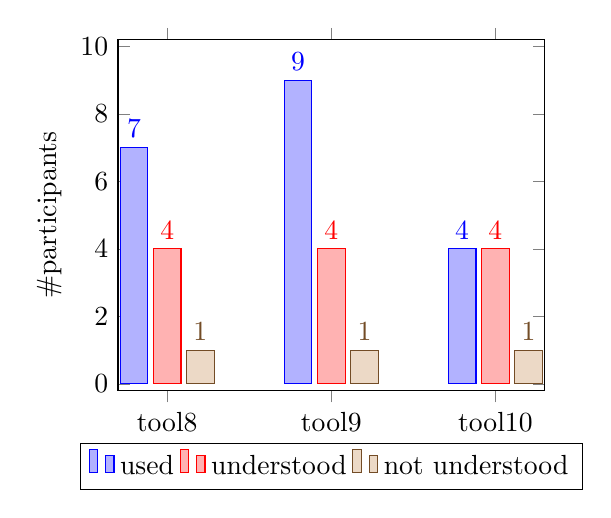
\begin{tikzpicture}
\begin{axis}[
    ybar,
    enlargelimits=0.15,
    legend style={at={(0.5,-0.15)},
      anchor=north,legend columns=-1},
    ylabel={\#participants},
    symbolic x coords={tool8,tool9,tool10},
    xtick=data,
    nodes near coords,
    nodes near coords align={vertical},
    ]
\addplot coordinates {(tool8,7) (tool9,9) (tool10,4)};
\addplot coordinates {(tool8,4) (tool9,4) (tool10,4)};
\addplot coordinates {(tool8,1) (tool9,1) (tool10,1)};
\legend{used,understood,not understood}
\end{axis}
\end{tikzpicture}

\end{document}